
\documentclass[conference]{IEEEtran}
\usepackage{cite}
\usepackage{amsmath,amssymb}
\usepackage{graphicx}
\usepackage{booktabs}
\usepackage{array}
\usepackage{url}
\usepackage{multirow}
\usepackage{balance}
\usepackage{caption}
\captionsetup{font=footnotesize}
\title{Enhanced 5G Handover Prediction over Real-Network RSRP Traces Using Lightweight Temporal Neural Representations}
\author{\IEEEauthorblockN{Mohammadali Mousavireineh and Astra Mousavireineh}
\IEEEauthorblockA{Independent Researchers\\
Corresponding author: mousavireineh@gmail.com}}
\begin{document}
\maketitle
\begin{abstract}
Reliable handover prediction is a key requirement for dense fifth-generation (5G) and beyond mobile networks, where frequent cell transitions can increase signaling load, interruption time, and the probability of radio link failure. A reproducible baseline has shown that long short-term memory (LSTM) forecasting of reference signal received power (RSRP), followed by a classical binary classifier, can support proactive handover triggering. However, nominal accuracy can be misleading when handover-trigger events are rare and the evaluation protocol depends on class balancing. This paper provides an enhanced and more conservative re-evaluation of temporal neural representations for real-network handover prediction. We compare the original LSTM-derived representation with a gated recurrent unit (GRU) representation and a temporal convolutional network (TCN) representation. For the downstream handover classifier, Random Forest, radial-basis SVM, k-nearest neighbors, and logistic regression are optimized using F1-oriented grid search. The processed ANATEL-derived feature bases contain 840 samples, of which only 19.64\% are positive handover-trigger examples. Under a stratified held-out test protocol, TCN+SVM achieves the best F1-score (0.4274) and balanced accuracy (0.6540), while LSTM+SVM remains close (F1 = 0.4237) and achieves the highest ROC-AUC (0.7050). The results suggest that lightweight temporal alternatives can improve or match LSTM-based handover representations under stricter evaluation, while also confirming that minority handover-event detection remains difficult in real-network traces.
\end{abstract}
\begin{IEEEkeywords}
5G, 6G, handover prediction, mobility management, LSTM, GRU, temporal convolutional network, RSRP, imbalanced classification.
\end{IEEEkeywords}

\section{Introduction}
Handover is the procedure by which a user equipment connection is transferred from one serving cell to another while maintaining service continuity. In dense 5G and beyond deployments, cell sizes shrink and coverage boundaries become more frequent, making mobility management more challenging. Incorrect handover timing can cause radio link failure, ping-pong effects, unnecessary signaling, interruption time, and degraded quality of experience. Machine learning is therefore increasingly investigated as a tool for proactive handover management, adaptive trigger configuration, and predictive cell selection \cite{mollel2021, thillaigovindhan2024}.

A recent baseline by Lima \emph{et al.} proposed a deep learning-based handover prediction pipeline in which an LSTM forecasts future RSRP samples and a downstream classifier predicts whether a handover trigger will occur \cite{lima2023}. The work is attractive because the authors released code and data, enabling reproducibility and extension. Nevertheless, in practical handover prediction, high overall accuracy can hide poor minority-class detection because handover-trigger events are rare compared with normal non-handover samples. A classifier that mostly predicts ``no handover'' can therefore appear accurate while missing the events that matter most operationally.

This paper revisits the LSTM-based handover prediction pipeline and strengthens it in two ways. First, it evaluates two alternative temporal representations, GRU and TCN, that are lighter or more parallelizable than stacked LSTMs. Second, it reports metrics that are more informative for imbalanced handover data, especially recall, F1-score, balanced accuracy, ROC-AUC, and confusion matrices. The main contributions are:
\begin{itemize}
\item a unified comparison of LSTM, GRU, and TCN-derived RSRP feature bases for real-network handover prediction;
\item a clearer algorithmic treatment of recurrent, gated, and convolutional temporal representations;
\item an F1-oriented grid-search comparison across Random Forest, SVM, KNN, and logistic regression classifiers;
\item a conservative held-out analysis that avoids relying only on nominal accuracy; and
\item a reproducible experimental structure that separates feature bases, classifier search, result tables, and manuscript figures.
\end{itemize}

\section{Previous Work}
Machine learning-based handover management has been surveyed extensively for 5G and beyond systems. Mollel \emph{et al.} reviewed supervised, unsupervised, and reinforcement learning approaches for handover management and identified data availability, generalization, and deployment constraints as major concerns \cite{mollel2021}. Recent surveys further emphasize that ultra-dense cells, heterogeneous access, and 6G-oriented architectures intensify the need for predictive mobility management \cite{thillaigovindhan2024}.

The closest baseline is the LSTM-based handover prediction method of Lima \emph{et al.} \cite{lima2023}. Their pipeline first forecasts future reference-signal measurements and then classifies the resulting sequence into handover or non-handover cases. This design is useful because it makes the intermediate signal prediction stage interpretable. However, downstream classification performance depends strongly on how class imbalance, sampling, and validation are handled.

Recent 6G-oriented work has also moved toward future serving-cell prediction and O-RAN-compatible deployment. Panitsas \emph{et al.} proposed a deep and transfer learning strategy for future serving-cell prediction and discussed integration with a near-real-time RAN Intelligent Controller as an xApp \cite{panitsas2024}. Karmakar \emph{et al.} studied adaptive time-to-trigger and hysteresis selection for intelligent mobility management \cite{karmakar2022}, while RANFusion provides a simulation environment for next-generation RAN handover scenarios \cite{ranfusion2024}.

On the modeling side, LSTM was introduced to address long-term dependency learning in recurrent neural networks \cite{hochreiter1997}. GRU later provided a simpler gated recurrent alternative with fewer gates and comparable sequence-modeling performance in many settings \cite{cho2014, chung2014}. TCNs use causal and dilated convolutions to model temporal dependencies and were shown by Bai \emph{et al.} to be strong alternatives to recurrent networks in sequence modeling tasks \cite{bai2018}. These properties motivate replacing or complementing LSTM-derived RSRP representations with GRU and TCN alternatives.

\section{Materials and Methods}
\subsection{Problem Formulation and Dataset}
This work uses processed feature bases derived from ANATEL real-network measurements released with the baseline handover prediction study \cite{lima2023}. For each sample, the downstream classifier receives a fixed-length temporal feature vector
\begin{equation}
\mathbf{x}_t = [\hat{r}_{t-49}, \hat{r}_{t-48}, \ldots, \hat{r}_t] \in \mathbb{R}^{50},
\end{equation}
where $\hat{r}_t$ denotes a predicted RSRP value generated by the corresponding temporal front end. The target label is
\begin{equation}
y_t = \begin{cases}
1, & \text{handover trigger} \\
0, & \text{no handover trigger}.
\end{cases}
\end{equation}
The processed dataset contains 840 samples: 675 non-handover samples and 165 handover-trigger samples. Therefore, the positive class ratio is only 19.64\%, making the task an imbalanced binary classification problem.

\begin{figure}[t]
\centering
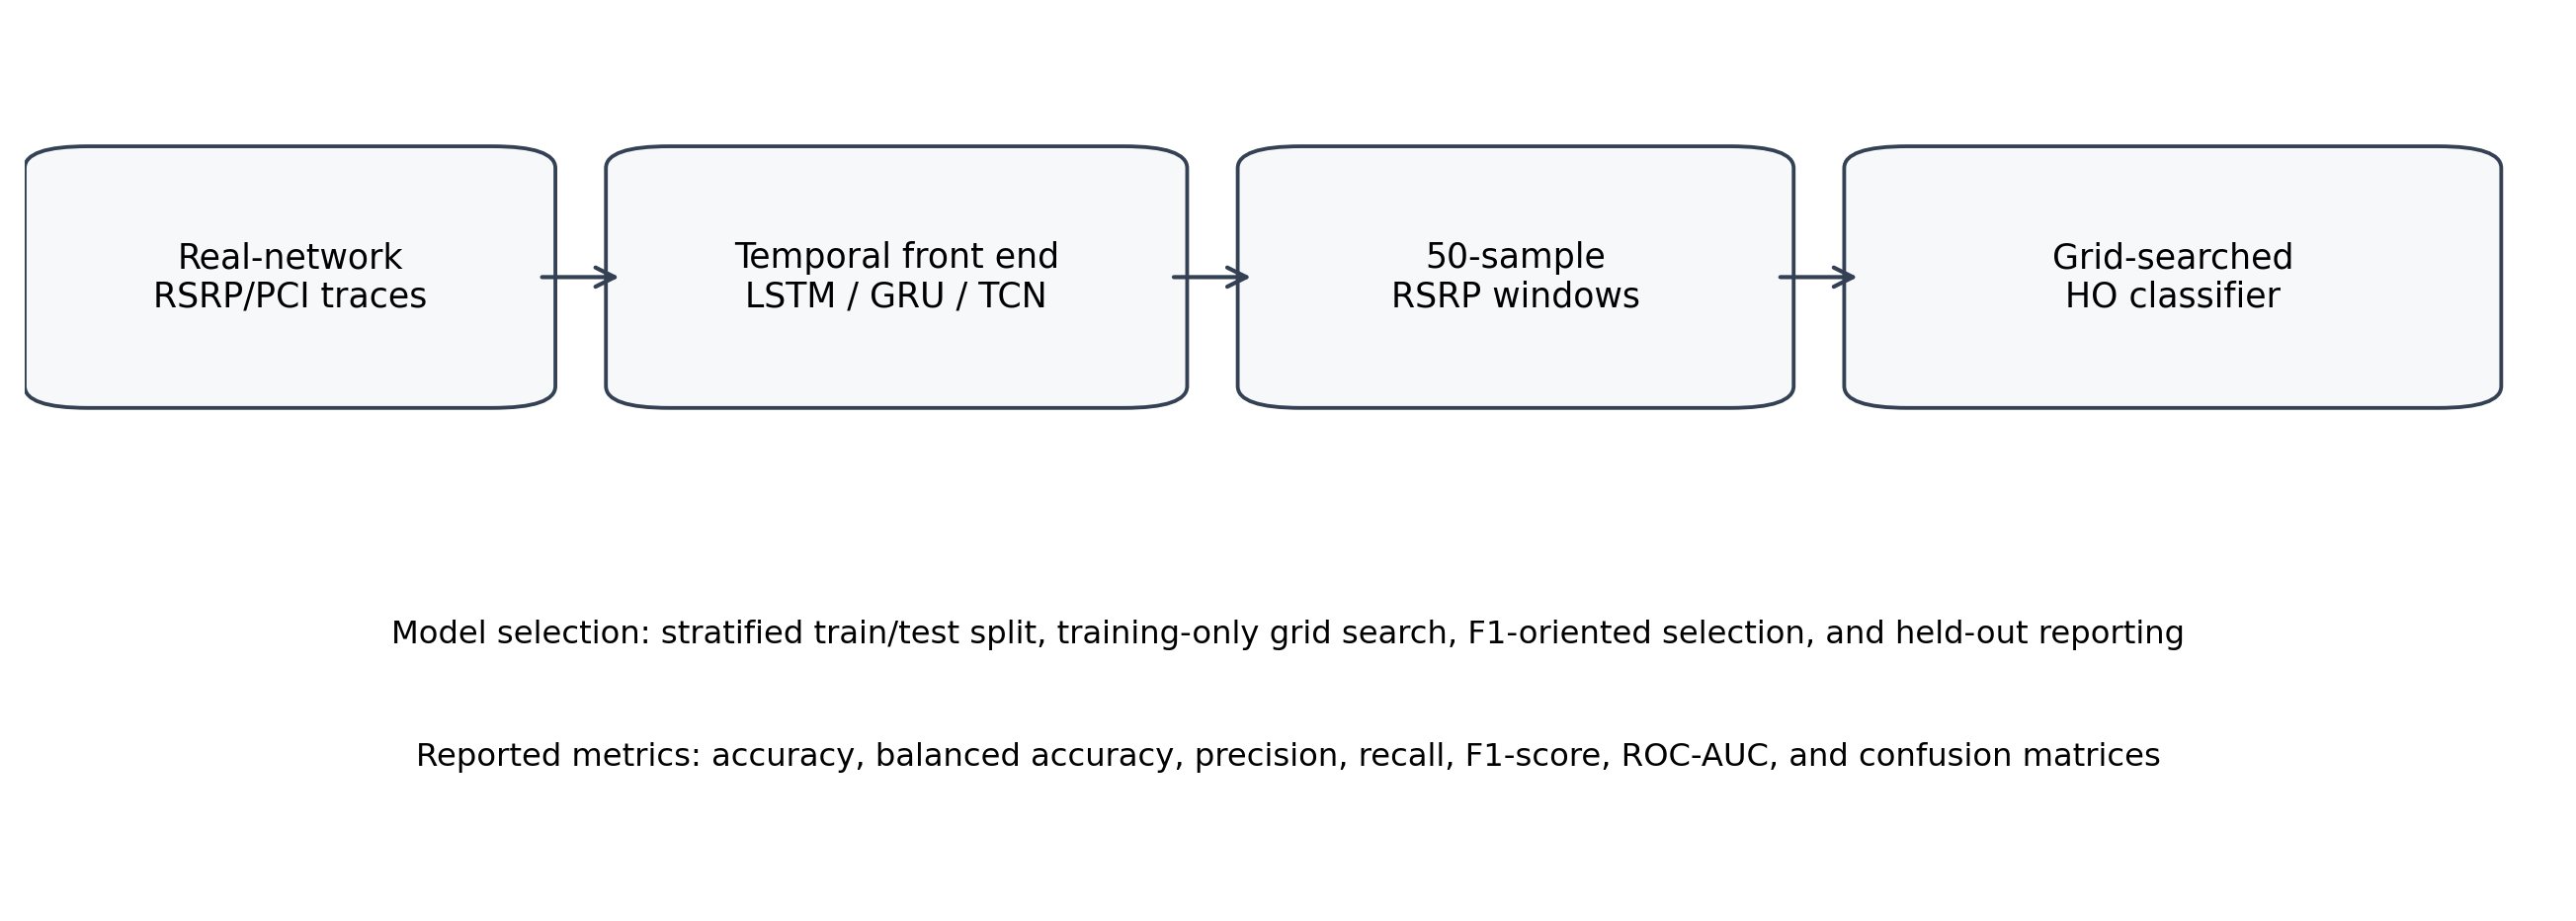
\includegraphics[width=\linewidth]{figures/fig1_pipeline.png}
\caption{Unified evaluation pipeline for comparing LSTM, GRU, and TCN-derived feature bases.}
\label{fig:pipeline}
\end{figure}

\begin{figure}[t]
\centering
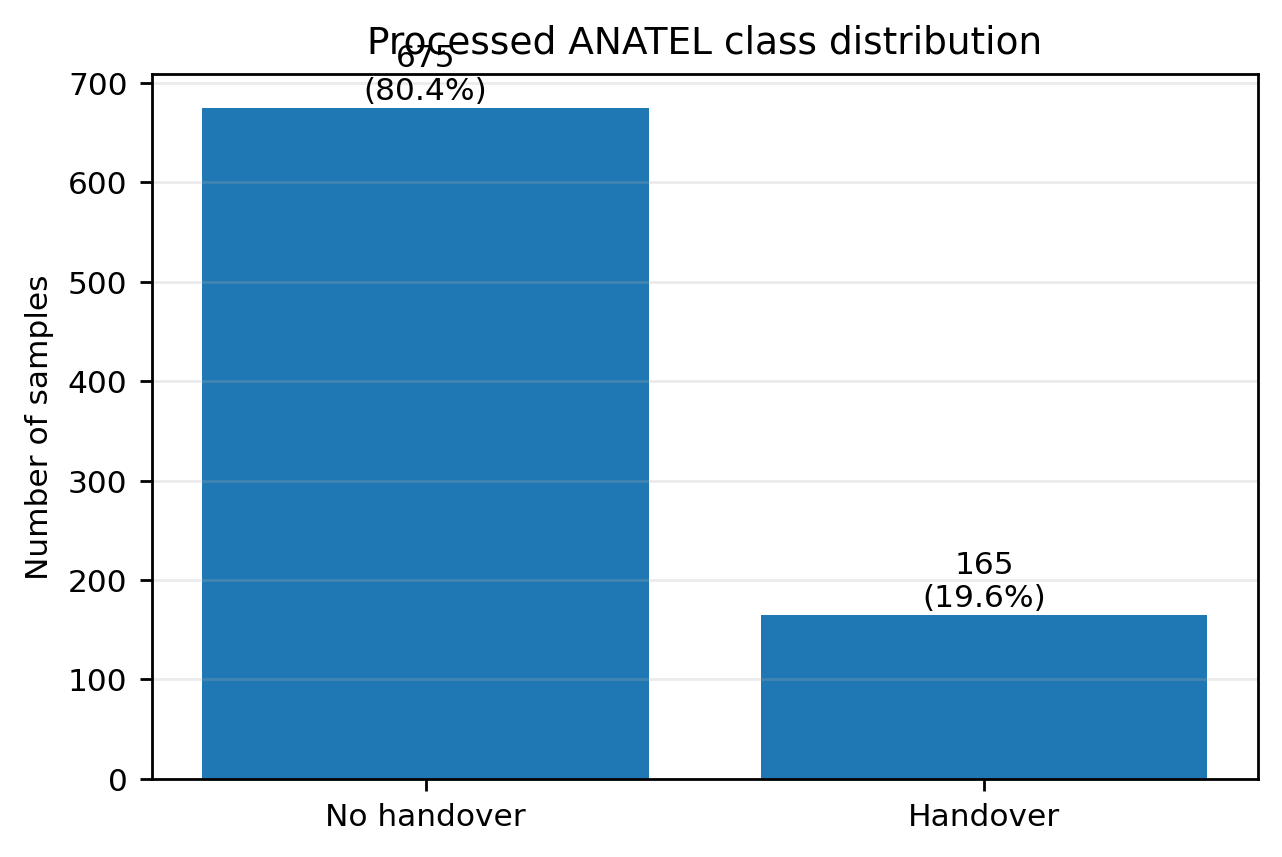
\includegraphics[width=0.86\linewidth]{figures/fig2_class_distribution.png}
\caption{Class distribution of the processed ANATEL feature bases. Handover-trigger samples form only 19.64\% of the data.}
\label{fig:classdist}
\end{figure}

\subsection{Temporal Representations}
\subsubsection{LSTM baseline}
LSTM is used as the baseline temporal representation because it was the core forecasting model in the original handover prediction pipeline. An LSTM cell uses input, forget, and output gates to control how information flows into the cell state and hidden state. A compact form is
\begin{align}
\mathbf{i}_t &= \sigma(\mathbf{W}_i \mathbf{x}_t + \mathbf{U}_i \mathbf{h}_{t-1} + \mathbf{b}_i), \\
\mathbf{f}_t &= \sigma(\mathbf{W}_f \mathbf{x}_t + \mathbf{U}_f \mathbf{h}_{t-1} + \mathbf{b}_f), \\
\mathbf{o}_t &= \sigma(\mathbf{W}_o \mathbf{x}_t + \mathbf{U}_o \mathbf{h}_{t-1} + \mathbf{b}_o), \\
\tilde{\mathbf{c}}_t &= \tanh(\mathbf{W}_c \mathbf{x}_t + \mathbf{U}_c \mathbf{h}_{t-1} + \mathbf{b}_c), \\
\mathbf{c}_t &= \mathbf{f}_t \odot \mathbf{c}_{t-1} + \mathbf{i}_t \odot \tilde{\mathbf{c}}_t, \\
\mathbf{h}_t &= \mathbf{o}_t \odot \tanh(\mathbf{c}_t).
\end{align}
LSTM is suitable for RSRP sequences because handover decisions depend on recent signal trends rather than on a single instantaneous measurement.

\subsubsection{GRU representation}
GRU was selected because it reduces the LSTM gating structure while retaining memory through update and reset gates. Its main equations can be written as
\begin{align}
\mathbf{z}_t &= \sigma(\mathbf{W}_z \mathbf{x}_t + \mathbf{U}_z \mathbf{h}_{t-1} + \mathbf{b}_z), \\
\mathbf{r}_t &= \sigma(\mathbf{W}_r \mathbf{x}_t + \mathbf{U}_r \mathbf{h}_{t-1} + \mathbf{b}_r), \\
\tilde{\mathbf{h}}_t &= \tanh(\mathbf{W}_h \mathbf{x}_t + \mathbf{U}_h(\mathbf{r}_t \odot \mathbf{h}_{t-1}) + \mathbf{b}_h), \\
\mathbf{h}_t &= (1-\mathbf{z}_t)\odot \mathbf{h}_{t-1} + \mathbf{z}_t\odot \tilde{\mathbf{h}}_t.
\end{align}
Compared with LSTM, GRU removes the separate memory cell and output gate. This makes it a natural candidate for lightweight handover prediction, especially when the target deployment is edge-oriented or near-real-time mobility control.

\subsubsection{TCN representation}
TCN was selected because it captures temporal dependencies using causal one-dimensional convolution rather than recurrent state updates. A dilated causal convolution can be represented as
\begin{equation}
\mathbf{y}_t = \sum_{k=0}^{K-1} \mathbf{w}_k \mathbf{x}_{t-dk},
\end{equation}
where $K$ is the kernel size and $d$ is the dilation factor. Dilation allows the model to cover a larger temporal receptive field without greatly increasing depth. Because convolutional operations can be parallelized across time windows, TCNs are attractive for scalable and low-latency inference.

\subsection{Downstream Classifiers}
Four classifier families are evaluated. The RBF-SVM maps inputs implicitly into a nonlinear feature space through the kernel
\begin{equation}
K(\mathbf{x}_i,\mathbf{x}_j) = \exp(-\gamma \|\mathbf{x}_i-\mathbf{x}_j\|^2),
\end{equation}
and was included because nonlinear decision boundaries may be needed when handover patterns are not linearly separable. Random Forest builds an ensemble of decision trees and predicts by majority vote, which improves robustness to noisy features. KNN classifies a test sample according to nearby training examples and provides a simple non-parametric baseline. Logistic regression estimates
\begin{equation}
P(y=1|\mathbf{x})=\sigma(\mathbf{w}^T\mathbf{x}+b),
\end{equation}
where $\sigma(\cdot)$ is the sigmoid function, and provides a linear probabilistic baseline.

\subsection{Evaluation Metrics}
Let TP, TN, FP, and FN denote true positives, true negatives, false positives, and false negatives, respectively. The reported metrics are
\begin{align}
\text{Accuracy} &= \frac{TP+TN}{TP+TN+FP+FN}, \\
\text{Precision} &= \frac{TP}{TP+FP}, \\
\text{Recall} &= \frac{TP}{TP+FN}, \\
\text{F1} &= \frac{2\cdot \text{Precision}\cdot \text{Recall}}{\text{Precision}+\text{Recall}}, \\
\text{Balanced Accuracy} &= \frac{1}{2}\left(\frac{TP}{TP+FN}+\frac{TN}{TN+FP}\right).
\end{align}
Accuracy is reported for comparison with previous work, but F1-score and recall are emphasized because the handover-trigger class is rare and operationally important.

\subsection{Evaluation Protocol}
The evaluation uses a stratified held-out split with 630 training samples and 210 test samples. All preprocessing that learns from data is fit only on the training set. Each classifier is wrapped in a pipeline with standardization where appropriate, and hyperparameters are selected using cross-validated grid search on the training set. F1-score is used as the model-selection criterion. SMOTE \cite{chawla2002} is relevant for class imbalance, but the primary reported results use the stricter non-SMOTE held-out protocol to avoid optimistic synthetic-sample effects on test performance.

\section{Results}
Table~\ref{tab:best} summarizes the best classifier found for each temporal feature base. The highest F1-score is obtained by the TCN feature base combined with an RBF-SVM classifier. LSTM+SVM performs very closely in F1-score and gives the highest ROC-AUC. GRU+SVM achieves a slightly lower F1-score and recall.

\begin{table*}[t]
\centering
\caption{Best held-out test results for each temporal feature representation.}
\label{tab:best}
\begin{tabular}{l l c c c c c c}
\toprule
Feature base & Classifier & Accuracy & Balanced acc. & Precision & Recall & F1 & ROC-AUC \\
\midrule
LSTM & SVM-RBF & 0.6762 & 0.6510 & 0.3247 & 0.6098 & 0.4237 & 0.7050 \\
GRU & SVM-RBF & 0.6714 & 0.6296 & 0.3108 & 0.5610 & 0.4000 & 0.7004 \\
TCN & SVM-RBF & 0.6810 & 0.6540 & 0.3289 & 0.6098 & 0.4274 & 0.6938 \\
\bottomrule
\end{tabular}
\end{table*}

\begin{figure*}[t]
\centering
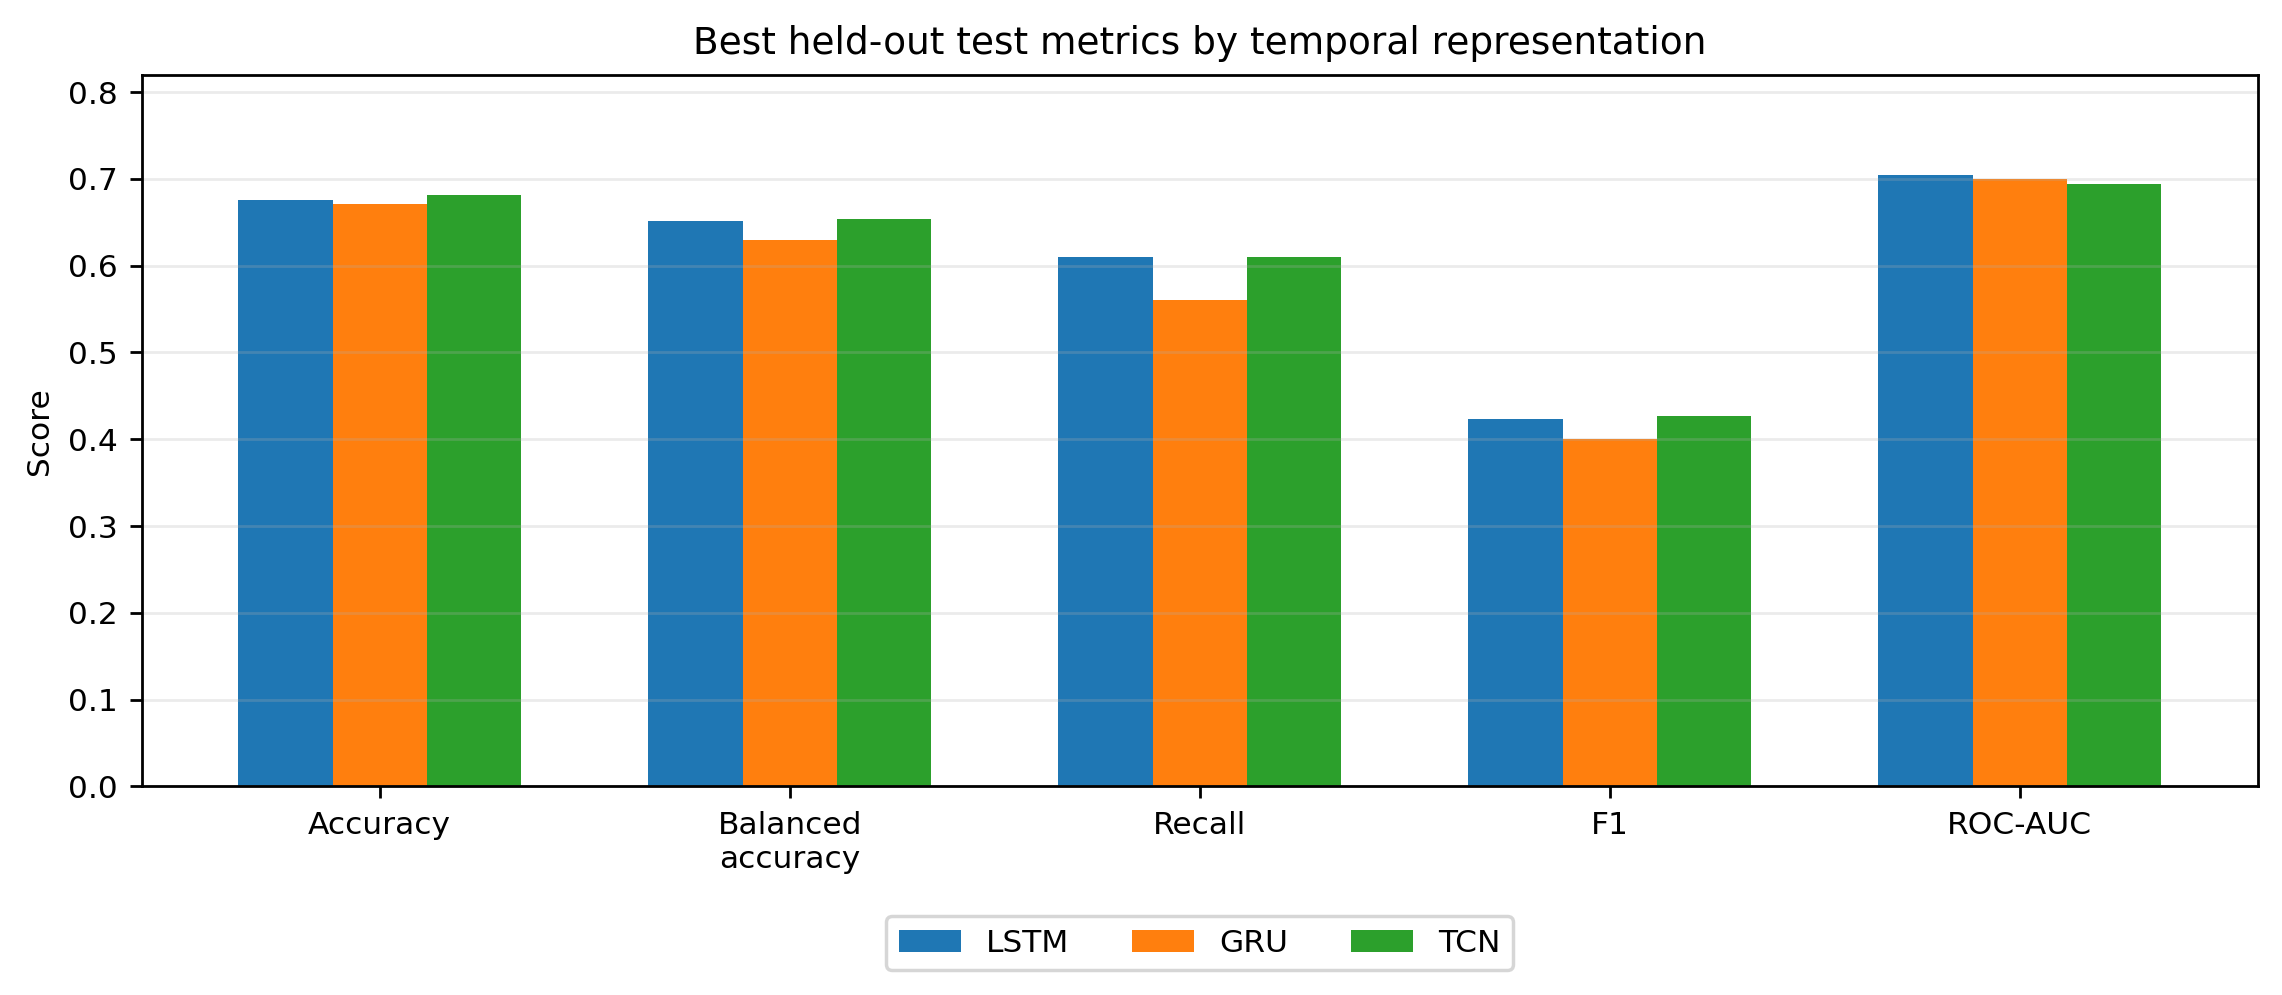
\includegraphics[width=0.92\textwidth]{figures/fig3_best_metrics.png}
\caption{Best held-out metrics by feature base. TCN and LSTM are close under the F1-oriented SVM setting.}
\label{fig:bestmetrics}
\end{figure*}

Table~\ref{tab:all} shows the classifier-level comparison. SVM is the most effective classifier family under the F1-oriented grid. KNN achieves higher overall accuracy for GRU and TCN, but lower recall and F1-score. This confirms that accuracy alone is not sufficient for handover-trigger detection in imbalanced data.

\begin{table*}[t]
\centering
\caption{Held-out results across classifier families. Rows are sorted by feature base and F1-score.}
\label{tab:all}
\begin{tabular}{l l c c c c c}
\toprule
Feature base & Classifier & Accuracy & Balanced acc. & Recall & F1 & ROC-AUC \\
\midrule
LSTM & SVM-RBF & 0.676 & 0.651 & 0.610 & 0.424 & 0.705 \\
LSTM & KNN & 0.752 & 0.569 & 0.268 & 0.297 & 0.702 \\
LSTM & RandomForest & 0.776 & 0.565 & 0.220 & 0.277 & 0.688 \\
LSTM & LogisticRegression & 0.462 & 0.444 & 0.415 & 0.231 & 0.446 \\
GRU & SVM-RBF & 0.671 & 0.630 & 0.561 & 0.400 & 0.700 \\
GRU & KNN & 0.762 & 0.593 & 0.317 & 0.342 & 0.704 \\
GRU & RandomForest & 0.762 & 0.547 & 0.195 & 0.242 & 0.692 \\
GRU & LogisticRegression & 0.467 & 0.438 & 0.390 & 0.222 & 0.434 \\
TCN & SVM-RBF & 0.681 & 0.654 & 0.610 & 0.427 & 0.694 \\
TCN & KNN & 0.762 & 0.593 & 0.317 & 0.342 & 0.711 \\
TCN & RandomForest & 0.786 & 0.590 & 0.268 & 0.328 & 0.704 \\
TCN & LogisticRegression & 0.510 & 0.446 & 0.341 & 0.214 & 0.451 \\
\bottomrule
\end{tabular}
\end{table*}

\begin{figure}[t]
\centering
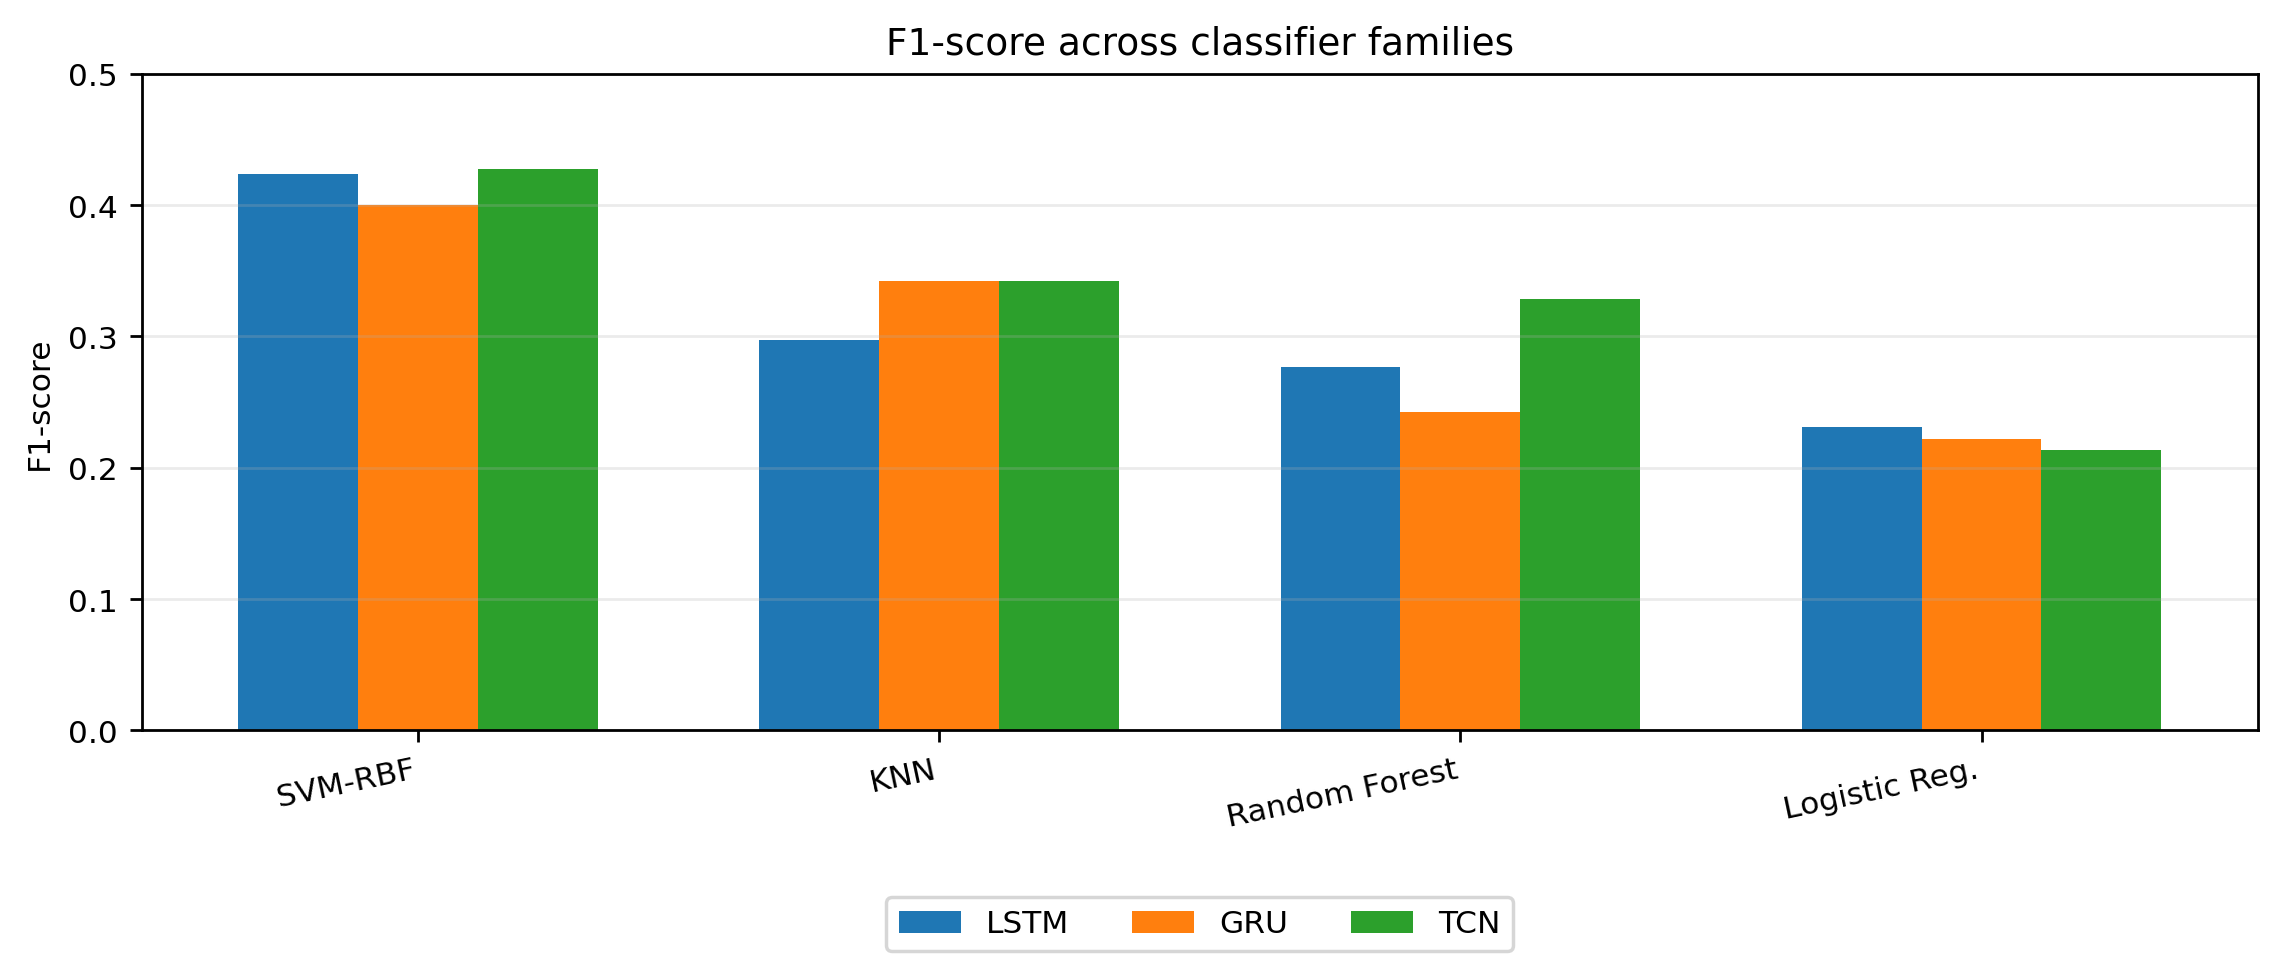
\includegraphics[width=\linewidth]{figures/fig4_classifier_f1.png}
\caption{F1-score comparison across classifier families.}
\label{fig:f1classifiers}
\end{figure}

\begin{figure*}[t]
\centering
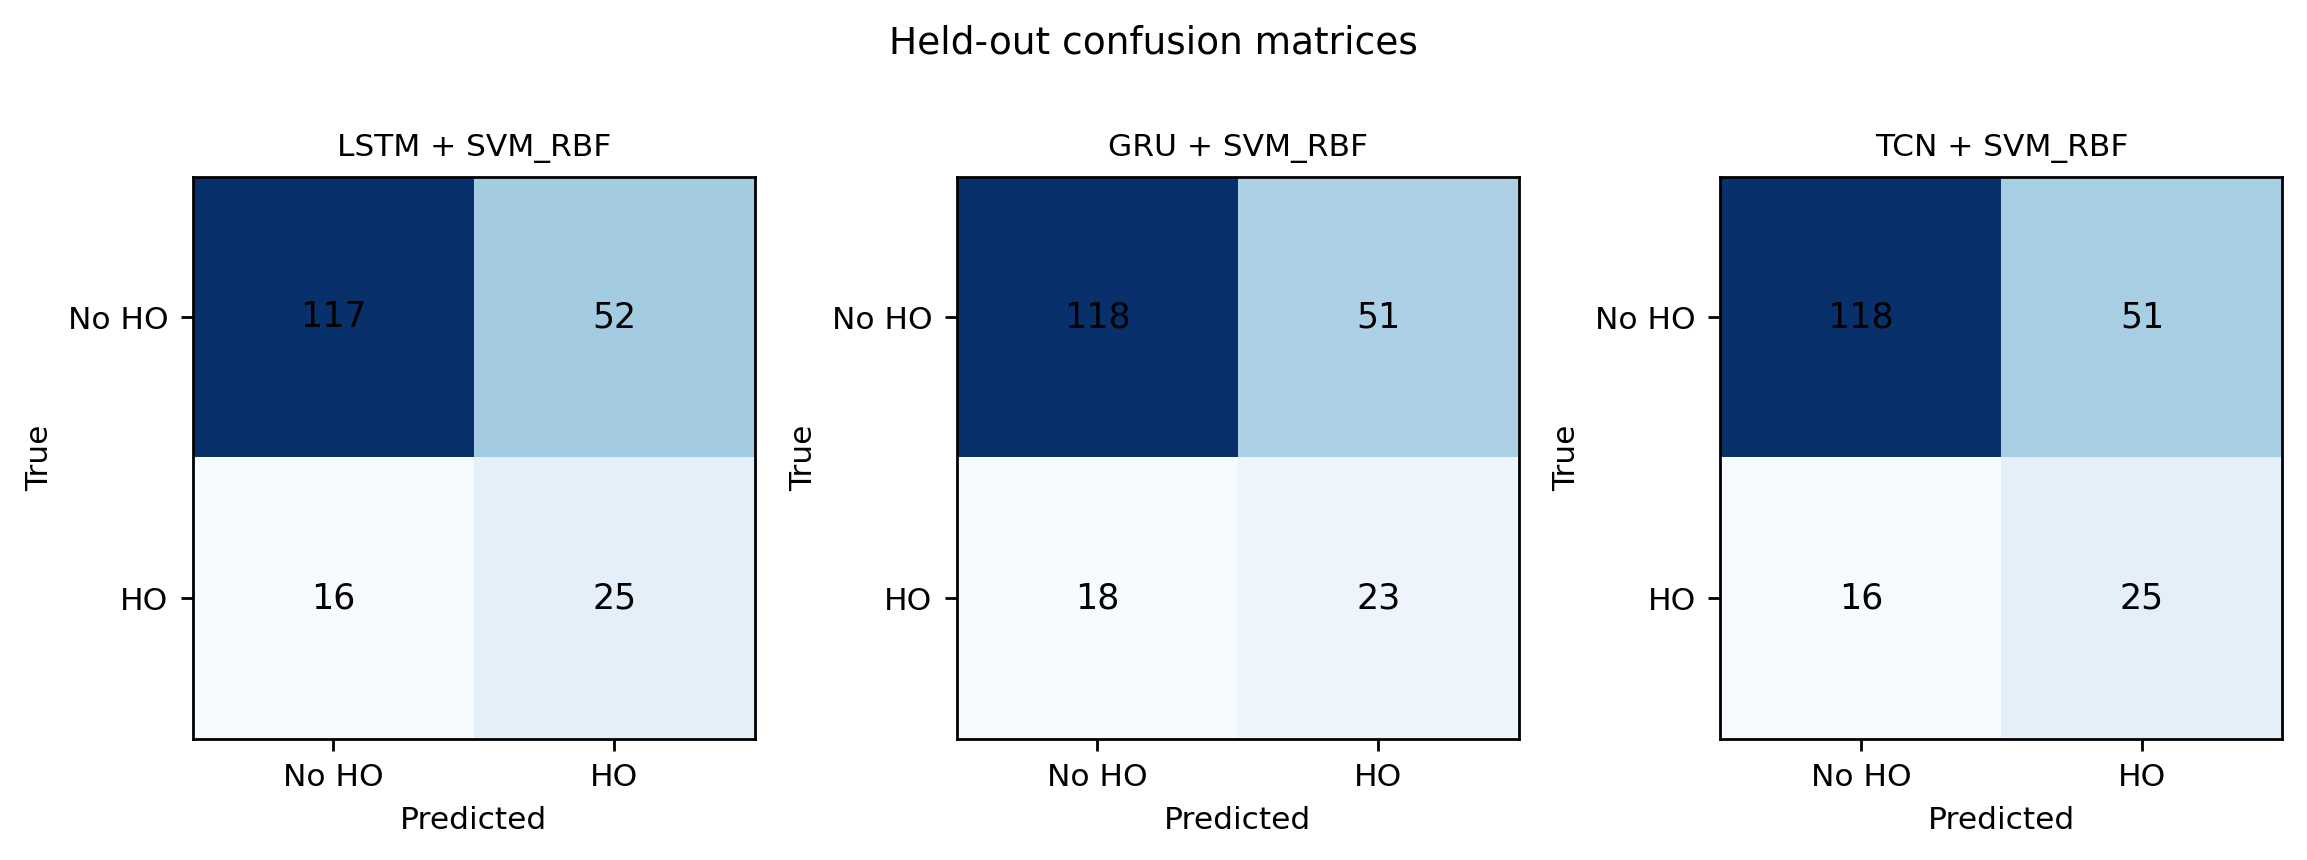
\includegraphics[width=0.92\textwidth]{figures/fig5_confusion_matrices.png}
\caption{Confusion matrices for the best classifier selected for each feature base. SVM improves handover recall but increases false positives.}
\label{fig:cms}
\end{figure*}

\section{Discussion}
The results show that the TCN feature base offers a small F1-score advantage over the LSTM baseline under the conservative held-out protocol. The margin is modest: TCN+SVM reaches F1 = 0.4274, while LSTM+SVM reaches F1 = 0.4237. Therefore, the appropriate conclusion is not that TCN decisively replaces LSTM, but that a convolutional temporal representation can match or slightly improve the LSTM-derived representation while offering an architecture that is naturally parallelizable.

The GRU representation does not outperform LSTM or TCN in the final held-out test, but it remains scientifically meaningful because it tests whether a simpler recurrent mechanism is sufficient for RSRP-derived handover prediction. Its lower F1-score suggests that reduced recurrent complexity alone may not be enough for this specific processed feature base. In contrast, TCN may benefit from local temporal pattern extraction over RSRP windows, which is consistent with the idea that handover risk is often signaled by short-term and medium-term signal trends.

The lower accuracy values compared with some baseline-paper reports should be interpreted carefully. In imbalanced handover prediction, accuracy can be inflated by majority-class behavior or by evaluation after balancing operations. The held-out protocol used here leaves the test set imbalanced and therefore emphasizes generalization to real minority-event detection. Under this setting, the SVM models improve recall to approximately 0.61 for LSTM and TCN, but precision remains near 0.33, indicating a trade-off between catching handover events and generating false alarms.

For operational mobility management, this trade-off is important. Missing a handover event can cause service degradation or interruption, while excessive false alarms can increase signaling and unnecessary handovers. Therefore, a practical deployment should optimize a cost-sensitive objective rather than a single generic metric. Depending on operator policy, recall may be prioritized in safety-critical or high-mobility scenarios, while precision may be prioritized when signaling overhead must be minimized.

\section{Limitations}
This study has several limitations. First, it uses processed feature bases rather than re-running all experiments from raw drive-test data. Second, the sample size is limited to 840 processed examples, and only 165 are positive handover-trigger cases. Third, the train-test split is stratified but not a full chronological deployment evaluation; future work should include temporal splits and cross-scenario validation. Fourth, the present contribution evaluates downstream classifiers on three temporal feature representations, but does not yet perform a full end-to-end neural classifier trained directly for the handover label. These limitations are explicitly stated to keep the claimed contribution proportional to the available evidence.

\section{Conclusion}
This paper enhanced and re-evaluated a reproducible handover prediction pipeline using LSTM, GRU, and TCN-derived RSRP feature bases on processed real-network ANATEL data. Under an F1-oriented held-out test protocol, TCN+SVM achieved the best F1-score of 0.4274 and balanced accuracy of 0.6540, while LSTM+SVM remained very close and achieved the highest ROC-AUC of 0.7050. The findings suggest that temporal convolutional representations can be competitive alternatives to recurrent baselines, but they also show that handover prediction on imbalanced real-network data remains difficult. Future work should evaluate end-to-end GRU/TCN classifiers, cost-sensitive thresholds, temporal deployment splits, and broader multi-cell or O-RAN-compatible scenarios.

\section*{Data and Code Availability}
The experiments were performed using processed feature bases and code organized in a reproducible repository structure containing data, model artifacts, experiment scripts, result CSV files, and generated figures. The raw ANATEL drive-test measurements are not redistributed in this manuscript package unless separately provided by the original source.

\balance

\begin{thebibliography}{99}
\bibitem{lima2023} J. P. S. H. Lima, A. A. M. de Medeiros, E. P. de Aguiar, and E. F. Silva, ``Deep Learning-Based Handover Prediction for 5G and Beyond Networks,'' in \emph{Proc. IEEE International Conference on Communications (ICC)}, 2023, doi: 10.1109/ICC45041.2023.10279195.
\bibitem{mollel2021} M. S. Mollel \emph{et al.}, ``A Survey of Machine Learning Applications to Handover Management in 5G and Beyond,'' \emph{IEEE Access}, 2021, doi: 10.1109/ACCESS.2021.3067503.
\bibitem{thillaigovindhan2024} S. K. Thillaigovindhan \emph{et al.}, ``A Comprehensive Survey on Machine Learning Methods for Handover Optimization in 5G Networks,'' \emph{Electronics}, vol. 13, no. 16, Art. no. 3223, 2024.
\bibitem{panitsas2024} I. Panitsas, A. Mudvari, A. Maatouk, and L. Tassiulas, ``Predictive Handover Strategy in 6G and Beyond: A Deep and Transfer Learning Approach,'' arXiv:2404.08113, 2024.
\bibitem{karmakar2022} R. Karmakar, G. Kaddoum, and S. Chattopadhyay, ``Mobility Management in 5G and Beyond: A Novel Smart Handover with Adaptive Time-to-Trigger and Hysteresis Margin,'' arXiv:2207.01706, 2022.
\bibitem{ranfusion2024} S. B. H. Natanzi and B. Tang, ``RANFusion: A Comprehensive Tool for Simulating Handover in Next-G RAN,'' arXiv:2405.19480, 2024.
\bibitem{hochreiter1997} S. Hochreiter and J. Schmidhuber, ``Long Short-Term Memory,'' \emph{Neural Computation}, vol. 9, no. 8, pp. 1735--1780, 1997, doi: 10.1162/neco.1997.9.8.1735.
\bibitem{cho2014} K. Cho \emph{et al.}, ``Learning Phrase Representations using RNN Encoder-Decoder for Statistical Machine Translation,'' in \emph{Proc. EMNLP}, 2014, pp. 1724--1734.
\bibitem{chung2014} J. Chung, C. Gulcehre, K. Cho, and Y. Bengio, ``Empirical Evaluation of Gated Recurrent Neural Networks on Sequence Modeling,'' arXiv:1412.3555, 2014.
\bibitem{bai2018} S. Bai, J. Z. Kolter, and V. Koltun, ``An Empirical Evaluation of Generic Convolutional and Recurrent Networks for Sequence Modeling,'' arXiv:1803.01271, 2018.
\bibitem{chawla2002} N. V. Chawla, K. W. Bowyer, L. O. Hall, and W. P. Kegelmeyer, ``SMOTE: Synthetic Minority Over-sampling Technique,'' \emph{Journal of Artificial Intelligence Research}, vol. 16, pp. 321--357, 2002, doi: 10.1613/jair.953.
\bibitem{breiman2001} L. Breiman, ``Random Forests,'' \emph{Machine Learning}, vol. 45, pp. 5--32, 2001, doi: 10.1023/A:1010933404324.
\bibitem{cortes1995} C. Cortes and V. Vapnik, ``Support-vector networks,'' \emph{Machine Learning}, vol. 20, pp. 273--297, 1995, doi: 10.1007/BF00994018.
\bibitem{sklearn2011} F. Pedregosa \emph{et al.}, ``Scikit-learn: Machine Learning in Python,'' \emph{Journal of Machine Learning Research}, vol. 12, pp. 2825--2830, 2011.
\end{thebibliography}

\end{document}
